% vim: set spell spelllang=es syntax=tex :

\documentclass[11pt,a4paper,spanish]{beamer}

\usepackage[spanish]{babel}

\usepackage[utf8]{inputenc}

\usepackage{graphicx}

\usepackage{subcaption}

\usepackage{url}

\usepackage{lineno} \linenumbers

\usepackage{babelbib}

\setlength{\parskip}{1.5mm}

\usetheme{Rochester}

\usecolortheme{dolphin}

\beamertemplatenavigationsymbolsempty

\begin{document}

\begin{frame}

\frametitle{Un sistema de visión global paralelo para fútbol de robots con fines
	educativos}

Autores:

\begin{itemize}

	\item Rodrigo Cañibano (rcanibano@fi.uncoma.edu.ar)
	
	\item Javier Balladini (javier.balladini@fi.uncoma.edu.ar)

	\item Eduardo Grosclaude (eduardo.grosclaude@fi.uncoma.edu.ar)

\end{itemize}

\mbox{
	
	\null\hspace{-0.1\paperwidth}
	
\includegraphics[width=0.1\paperwidth]{logos/fai.pdf}
	\hspace{0.8\paperwidth}
	\includegraphics[width=0.1\paperwidth]{logos/uncoma.pdf}
	
}

\end{frame}

\begin{frame}

\begin{itemize}

\item Introducción:

\begin{itemize}

	\item ¿Que es un sistema de visión global para fútbol de robots?

	\item ¿Por que un sistema con fines educación?

	\item ¿Por que paralelo?

\end{itemize}

\item Descripción del sistema:

\begin{itemize}

	\item Oportunidades de paralelismo.

	\item División de los datos.

	\item Arquitectura del sistema.

	\item Experimentación y resultados.

	\item Uso educativo.

\end{itemize}

\item Conclusiones y trabajos futuros

\end{itemize}

\end{frame}

\begin{frame}

\frametitle{¿Que es fútbol de robots?}

	Nos enfocamos en la liga de tamaño pequeño \emph{SSL} de la
	\emph{RoboCup}:

\begin{itemize}

	\item Dos equipos de seis robots cada uno.

	\item Una computadora por equipo controla los robots.

	\item Sistema de visión global (\emph{SVG}) compartido por ambos
		equipos.

\end{itemize}

\end{frame}

\begin{frame}

\frametitle{Arquitectura del \emph{SVG} para la \emph{SSL}}

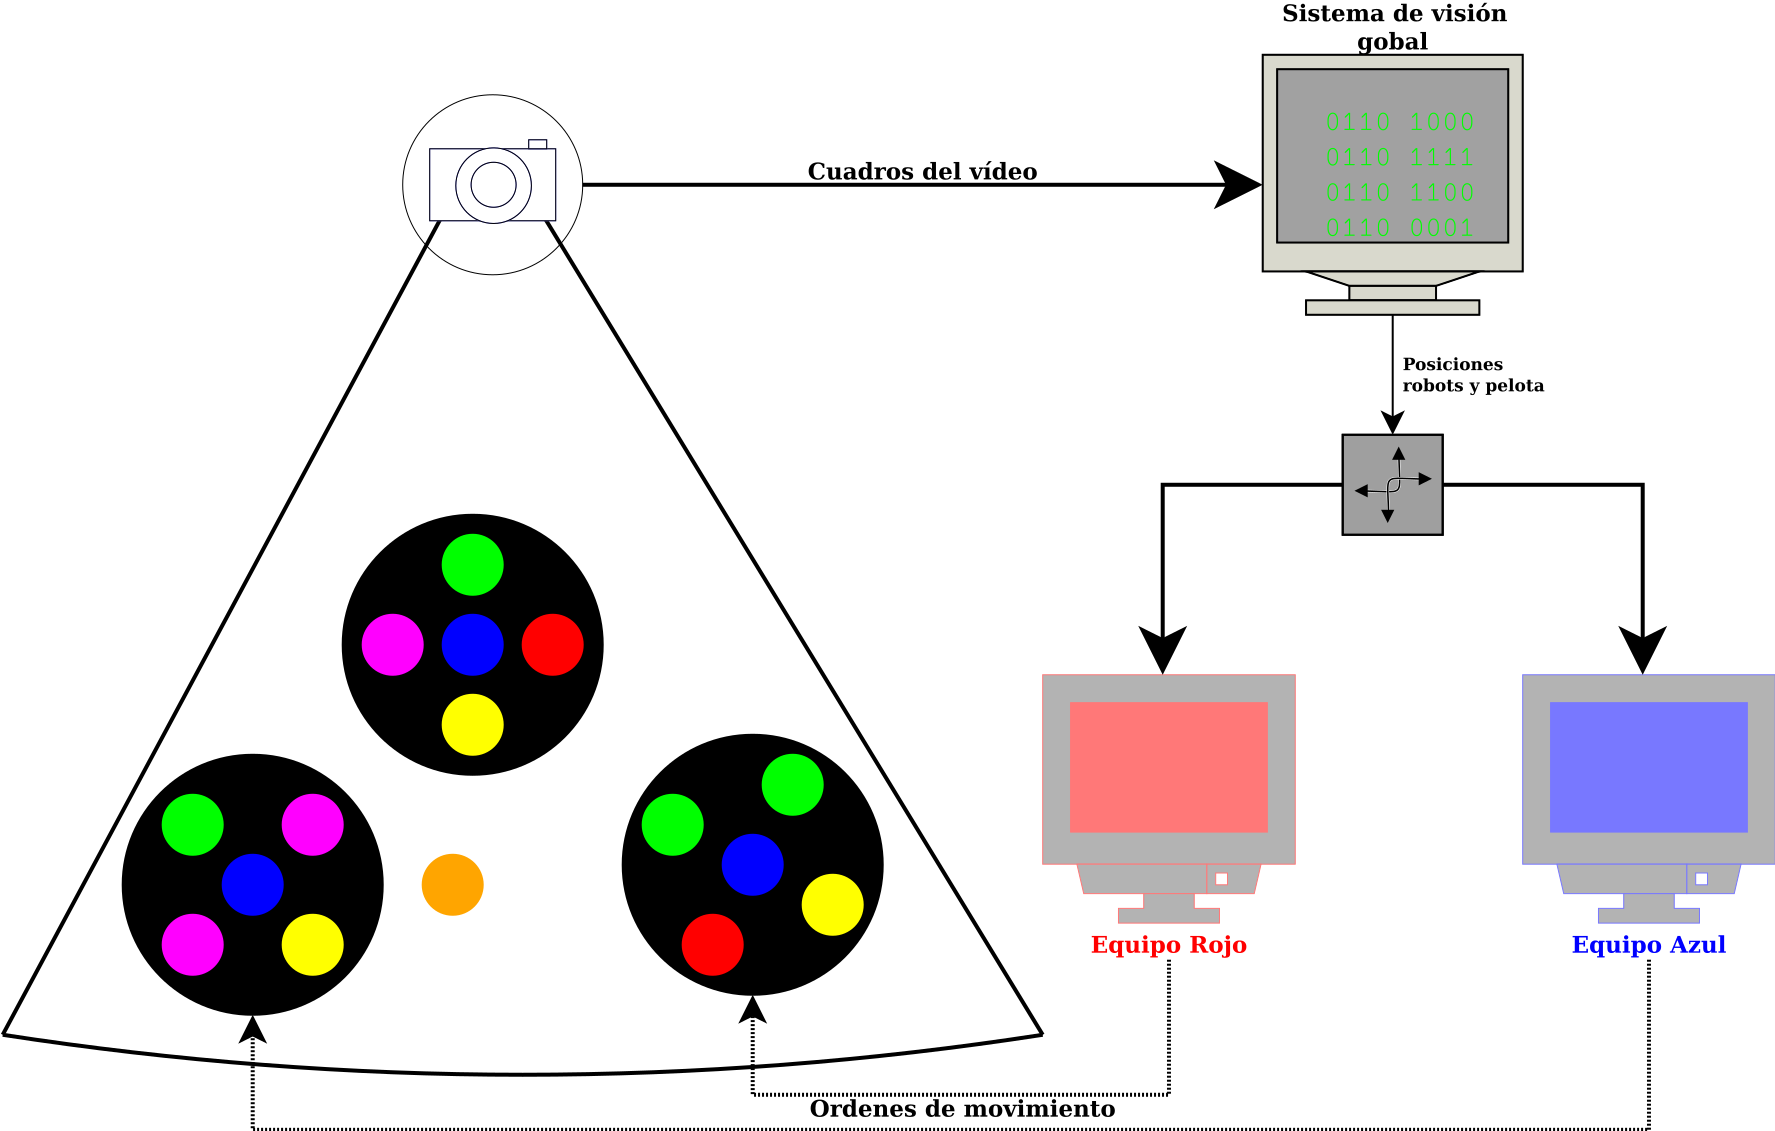
\includegraphics[width=\textwidth]{img/sistemaVG.pdf}

\end{frame}

\begin{frame}

\frametitle{Software de \emph{SVG} de la \emph{SSL}}

\begin{itemize}

	\item Problema ideal para la introducción a la visión por computadora.

\end{itemize}

Pero:

\begin{itemize}

	\item Para la \emph{RoboCup} el \emph{SVG} es un problema ya
		solucionado: \emph{SSL-VISION}
	
	\item \emph{SSL-VISION} plugins muy avanzados para su uso como
		herramienta educativa.

	\item El sistema actual no es escalable, pero el tamaño de la cancha
		sigue aumentando.

\end{itemize}

\end{frame}

\begin{frame}

\frametitle{Objetivos}

Desarrollar un \emph{SVG} paralelo para fútbol de robots con fines educativos:

\begin{itemize}

	\item Plugins mas sencillos, aunque sean menos eficientes.

	\item Que sea escalable.

	\item Con un framework orientado al desarrollo de aplicaciones
		paralelas, que permita explorar distintas técnicas de
		paralelismo.

\end{itemize}

\end{frame}

\begin{frame}

\frametitle{Oportunidades de paralelismo}

\begin{itemize}

	\item Paralelismo dentro del cuadro.
		
\begin{itemize}

	\item Procesar distintas partes del cuadro en paralelo.

\end{itemize}

	\item Paralelismo entre cuadros.

\begin{itemize}

	\item Procesar distintos cuadros en paralelo.

\end{itemize}

\end{itemize}

\end{frame}

\begin{frame}

\frametitle{Consideraciones para la fragmentación del cuadro}

\begin{figure}[h]

	\centering
	
	
\includegraphics[width=0.45\textwidth]{img/areaTooSmall.pdf}~
	
\includegraphics[width=0.45\textwidth]{img/areaPerfect.pdf}

\end{figure}

\end{frame}

\begin{frame}

\frametitle{Consideraciones para la fragmentación del cuadro}

\begin{figure}[h]

	
\includegraphics[width=0.40\textwidth]{img/fragmentos1.pdf}~
	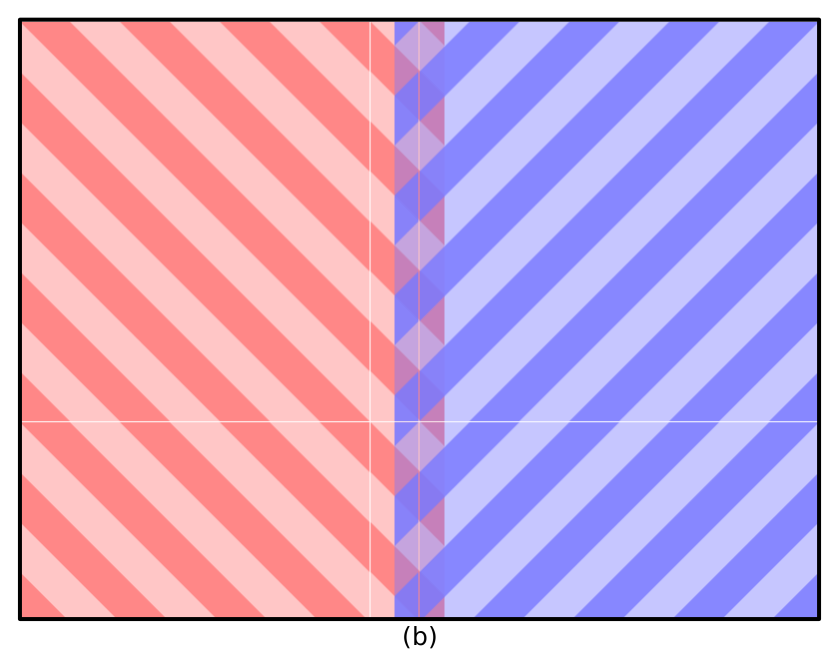
\includegraphics[width=0.40\textwidth]{img/fragmentos2.pdf}

	\includegraphics[width=0.40\textwidth]{img/fragmentos5.pdf}~
	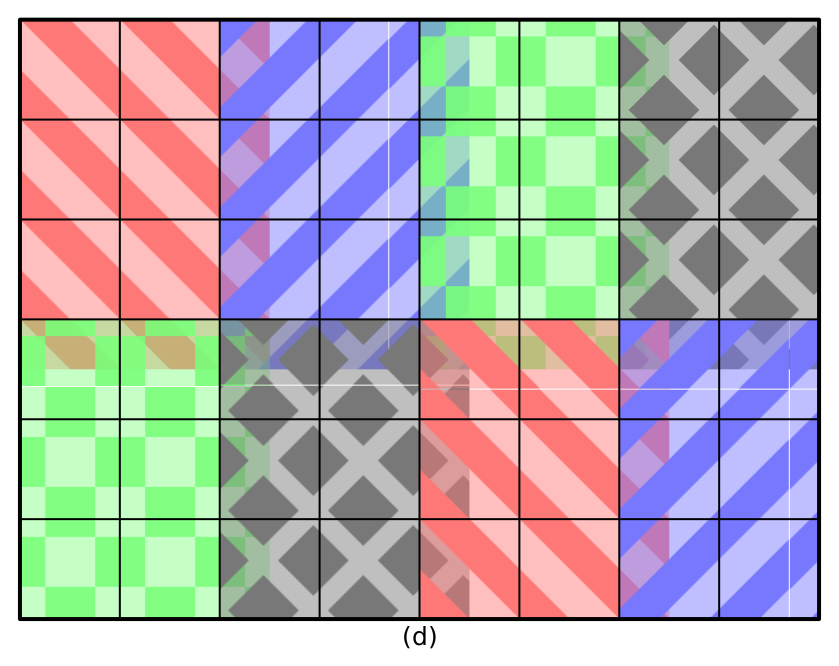
\includegraphics[width=0.40\textwidth]{img/fragmentos8.pdf}

\end{figure}

\end{frame}

\begin{frame}

\frametitle{Arquitectura del sistema}

\begin{itemize}

	\item Cada tarea estática tiene un hilo de ejecución.

	\item Existe un pool de hilos de ejecución para las tareas dinámicas.

\end{itemize}

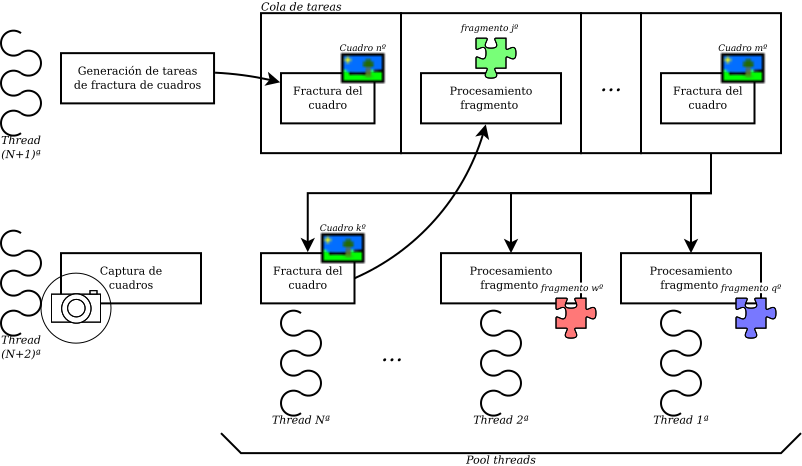
\includegraphics[width=\textwidth]{img/hilos.pdf}

\end{frame}

\begin{frame}

\frametitle{Experimentación}

Buscamos:

\begin{itemize}

	\item \emph{FPS} y luego Retardo de cuadro

\end{itemize}

Plataforma experimental:

\begin{itemize}

	\item Intel Xeon E5-2630 (2,3GHz) de 6 núcleos con multithreading
		simultáneo de dos vías (12 núcleos virtuales)

	\item Memoria cache 15MiB L3, 256KiB L2, 32KiB L1i, 32KiB L1d

\end{itemize}

Variables:

\begin{itemize}

	\item Dos vídeos 1280x720px y 800x600px.

	\item Cantidad de hilos para tareas dinámicas.

	\item de 1 a 12.

	\item Cantidad de fragmentos.

	\item de 1 a 24.

\end{itemize}

\end{frame}

\begin{frame}

\frametitle{Resultados: \emph{FPS} vídeo 1280x720px}

\includegraphics[width=\textwidth]{img/1280x720_fps.pdf}

\end{frame}

\begin{frame}

\frametitle{Resultados: \emph{FPS} números primos}

\includegraphics[width=\textwidth]{img/primos_fps.pdf}

\end{frame}

\begin{frame}

\frametitle{Resultados: Fallos de cache por cuadro}

\includegraphics[width=\textwidth]{img/cache_fallos.pdf}

\end{frame}

\begin{frame}

\frametitle{Resultados: Escalabilidad \emph{FPS}}

\includegraphics[width=\textwidth]{img/1280x720_bestfps.pdf}

\end{frame}

\begin{frame}

\frametitle{Retardo de cuadro por cada \emph{FPS}}

\includegraphics[width=\textwidth]{img/1280x720_tFPS.pdf}

\end{frame}

\begin{frame}

\frametitle{Usos educativos}


\begin{itemize}
	
	\item Se puede experimentar con distintas estrategias de división.

	\item Tanto en cantidad de partes.

	\item Cambiando la forma de fractura.

	\item El modificar y agregar plugins. Posiblemente adaptándolo a otro
		dominio.
	
\end{itemize}

\end{frame}

\begin{frame}

\frametitle{Conclusiones}


\begin{itemize}

	\item Se desarrollo un sistema de visión global para fútbol de robots
		que puede ser utilizado como herramienta educativa.

	\item Se analizaron los comportamientos bajo distintas configuraciones.

\end{itemize}

Trabajos futuros:

\begin{itemize}
	
	\item Agregar una interfaz gráfica que permita visualizar los resultados
		de los plugins.

	\item Seguir trabajando sobre los plugins para hacerlos mas accesibles.

\end{itemize}

\end{frame}

\begin{frame}

	\frametitle{¡Muchas Gracias!}

\end{frame}

\bibliographystyle{babplain}

\bibliography{biblio}

\end{document}
